\documentclass{article}
%\usepackage{enumitem}
\usepackage[table]{xcolor}
\usepackage{listings}
\usepackage{amsfonts}
\usepackage{latexsym}
\usepackage{fullpage}
\usepackage{graphicx}
%\usepackage{paralist}
\usepackage{tikz-timing}
\usepackage{tabto}
\usepackage[utf8]{inputenc}
\usepackage[T1]{fontenc}
\usepackage{filecontents}
\usepackage[backend=biber,style=ieee]{biblatex}
\usepackage{caption}
\usepackage{subcaption}
\usepackage[brazilian]{babel}
\lstset{language=C}

\graphicspath{{images/}}

% Default margins are too wide all the way around. I reset them here
\setlength{\topmargin}{-.5in}
\setlength{\textheight}{9in}
\setlength{\oddsidemargin}{.125in}
\setlength{\textwidth}{6.25in}

% Defining references here

\begin{filecontents}{\jobname.bib}
@article{singh2014,
author = {Dhananjay, Singh and Gaurav, Tripathi},
year = {2014},
month = {03},
pages = {},
title = {A Survey of Internet-of-Things: Future Vision, Architecture, Challenges and Services},
journaltitle = {2014 IEEE World Forum on Internet of Things, WF-IoT 2014}
}
@online{arduinoblog,
author = {Arduino},
title = {Arduino Blog},
year = {2017},
url = {https://blog.arduino.cc},
OPTnote = {Acessado em 24 de Abril de 2017}
}
@article{santanna2012,
author = {Francisco Sant’Anna and
Noemi de La Rocque Rodriguez and
Roberto Ierusalimschy},
title = {CÉU: Embedded, Safe, and
Reactive},
journaltitle = {Monografias em Ciência da Computação},
year = {2012},
volume = {9},
issn = {0103-9741}
}
@online{githubceuarduino,
author = {Francisco Sant'Anna},
title = {GitHub Céu-Arduino},
year = {2017},
url = {https://github.com/fsantanna/ceu-arduino},
note = {Acessado em 24 de Abril de 2017}
}
@article{wortmann2015,
author = {Felix Wortmann and Kristina Flütcher},
year = {2015},
pages = {221-224},
title = {Internet of Things - Technology and Value Added},
journaltitle = {Business \& Information Systems Engineering},
volume = {57},
issue = {3}
}
@periodical{chui2010,
editor = {Michael Chui and Markus Löffer and Roger Roberts},
title = {The Internet of Things},
year = {2010},
series = {McKinsey Quarterly},
month = {Março},
url = {https://www.mckinsey.com/industries/high-tech/our-insights/the-internet-of-things}
}
@ARTICLE{edwards1997, 
author={S. Edwards and L. Lavagno and E. A. Lee and A. Sangiovanni-Vincentelli}, 
journal={Proceedings of the IEEE}, 
title={Design of embedded systems: formal models, validation, and synthesis}, 
year={1997}, 
volume={85}, 
number={3}, 
pages={366-390}, 
keywords={application specific integrated circuits;computer architecture;formal specification;formal verification;logic design;real-time systems;systems analysis;ASIC;application-specific integrated circuits;concurrent design process;embedded software;embedded systems design;formal models;formal validation;heterogeneous systems;reactive real-time system design;specification;Application software;Application specific integrated circuits;Computer architecture;Consumer electronics;Embedded computing;Embedded system;Hardware;Microcontrollers;Real time systems;Safety}, 
doi={10.1109/5.558710}, 
ISSN={0018-9219}, 
month={Mar},}
@online{githubceu,
author = {Francisco Sant'Anna},
title = {GitHub Céu},
year = {2017},
url = {https://github.com/fsantanna/ceu},
note = {Acessado em 24 de Abril de 2017}
}
@manual{atmegadatasheet,
author = {AtMel},
title = {AtMel ATmega328/P DATASHEET},
year = {2016},
organization = {ATMel},
}

\end{filecontents}

\addbibresource{\jobname.bib}

% End defining references

\begin{document}

\begin{titlepage}

\newcommand{\HRule}{\rule{\linewidth}{0.5mm}} % Defines a new command for the horizontal lines, change thickness here

\center % Center everything on the page
 
%----------------------------------------------------------------------------------------
%	HEADING SECTIONS
%----------------------------------------------------------------------------------------

\textsc{\LARGE Pontifícia Universidade Católica do Rio de Janeiro}\\[1.5cm] % Name of your university/college
\textsc{\Large Projeto Final de Graduação de Engenharia da Computação}\\[0.5cm] % Minor heading such as course title

\textsc{\large Departamento de Informática - DI \\ Centro Técnico Científico - CTC \\ Curso de Engenharia da Computação}\\[0.5cm] % Major heading such as course name


%----------------------------------------------------------------------------------------
%	TITLE SECTION
%----------------------------------------------------------------------------------------

\HRule \\[0.4cm]
{ \huge \bfseries Aplicação em Sistemas Distribuídos
utilizando biblioteca e driver próprios,
baseados em interrupções desenvolvido
em Céu para o microcontrolador Arduino}\\[0.4cm] % Title of your document
\HRule \\[1.5cm]
 
%----------------------------------------------------------------------------------------
%	AUTHOR SECTION
%----------------------------------------------------------------------------------------

\begin{minipage}{0.4\textwidth}
\begin{flushleft} \large
\emph{Aluno:}\\
Guilherme \textsc{Simas} % Your name
\end{flushleft}
\end{minipage}
~
\begin{minipage}{0.4\textwidth}
\begin{flushright} \large
\emph{Orientador:} \\
Ana \textsc{Lúcia de Moura} % Supervisor's Name
\end{flushright}
\end{minipage}\\[4cm]

% If you don't want a supervisor, uncomment the two lines below and remove the section above
%\Large \emph{Author:}\\
%John \textsc{Smith}\\[3cm] % Your name

%----------------------------------------------------------------------------------------
%	DATE SECTION
%----------------------------------------------------------------------------------------

{\large \today}\\[3cm] % Date, change the \today to a set date if you want to be precise

%----------------------------------------------------------------------------------------
%	LOGO SECTION
%----------------------------------------------------------------------------------------

%\includegraphics{Logo}\\[1cm] % Include a department/university logo - this will require the graphicx package
 
%----------------------------------------------------------------------------------------

\vfill % Fill the rest of the page with whitespace

\end{titlepage}

\newpage % Dedicatória

\begin{flushright}

\vspace*{\fill}

\textit{\LARGE Agradecimentos estarão descritos nesse bloco de texto. Caso o bloco de texto seja grande demais espera-se que ele pule linhas e continue se guiando pela margem direita}

\vspace*{\fill}

\end{flushright}

\newpage

\tableofcontents{}

\newpage

\section{Introdução}	


\tab Atualmente existe uma grande variedade de estudos e soluções no âmbito da Internet das Coisas
promovidos por empresas de tecnologia da informação, mostrando que o conceito pode ser
implementado e, embora não tenha uma presença evidente no dia-a-dia, está em constante
desenvolvimento e em processo de adequação. Existem várias definições do termo “Internet das
Coisas”, porém a grande maioria delas compartilha o foco em aplicações escaláveis que envolvem a cooperação entre múltiplas partes em busca do objetivo em comum.  \cite{singh2014}
Para viabilizar a escabilidade prevista nas aplicações em Internet das Coisas, são necessárias unidades
computacionais de custo baixo e consumo eficiente de energia. Por esse motivo microcontroladores
são outra parte vital do desenvolvimento de soluções, apresentando, entre outras vantagens, uma
facilidade na programação devido a bibliotecas e drivers já implementados e disponibilizados.
Microcontroladores são capazes de processamento de dados por possuírem processadores e de
serem facilmente integrados com sensores e atuadores, possuindo hardware especializado para
interfacear com esses componentes.
\par Muitas APIs (conjuntos de rotinas, protocolos e ferramentas para desenvolvimento de software para
uma plataforma) fornecidas por microcontroladores incluem rotinas que causam um bloqueio na
aplicação, ou seja, enquanto está realizando a chamada correspondente àquela funcionalidade, o
software entra em um estado onde realiza tarefas virtualmente inúteis até que o hardware conclua sua
parte. Esse comportamento é indesejável visto que a aplicação desperdiça tempo aguardando o
hardware enquanto poderia estar realizando outras tarefas como, por exemplo, um processamento de
dados recebidos por uma mensagem, ou a troca de mensagens em si. Essa ineficiência marca um
desperdício de tempo e consumo de energia.
\par O bloqueio de aplicações é um desafio enfrentado frequentemente em aplicações que envolvem
sistemas nos quais o tempo de processamento ou reação a estímulos externos é pertinente ao
funcionamento da aplicação. O paradigma de programação orientada a eventos é muitas vezes
utilizado como abordagem nessas situações. Em uma aplicação orientada a eventos, o sistema segue
seu fluxo normal até a chegada de um “evento”, como a chegada de uma mensagem, ou a conclusão
de um trabalho por parte do hardware. Esse paradigma permite estruturar a aplicação de forma a evitar que
quaisquer estímulos sejam ignorados involuntariamente ou que ciclos computacionais
sejam desperdiçados. Essa estruturação, porém, introduz uma espécie de paralelismo e imprevisibilidade no
fluxo de execução da aplicação que é de difícil representação por linguagens utilizadas no meio atualmente.
\par Esse trabalho propõe reimplementar drivers e bibliotecas do microcontrolador Arduino, que atualmente causam
bloqueio da aplicação, de forma a que esse bloqueio não ocorra mais. A abordagem utilizada nesse
desenvolvimento será do uso de interrupções suportadas por hardware especializado com orientação a
eventos. Com esses fatores em mente, a linguagem escolhida para esse desenvolvimento foi Céu\cite{santanna2012}, uma linguagem reativa orientada a eventos desenvolvida na PUC, em conjunto com um kit da linguagem para desenvolvimento para Arduino, chamado Céu-Arduino\cite{githubceuarduino}. Os
resultados desse desenvolvimento serão publicados na página open-source de desenvolvimento do
kit, para que futuros desenvolvedores possam fazer uso de tais módulos em suas próprias aplicações
e objetivos.
\par Por fim, será desenvolvida uma aplicação em Sistemas Distribuídos para exemplificar a pertinência
dos módulos desenvolvidos. A aplicação consistirá em uma rede de sensores e atuadores na
plataforma Arduino, utilizando troca de mensagens. Alguns exemplos de aplicações que satisfazem
os requisitos e objetivos são: Um sistema de iluminação inteligente; um sistema de irrigação
monitorada; um controlador de tráfego. Esse trabalho tem como meta servir como uma contribuição
para a comunidade desenvolvedora de sistemas embarcados e de aplicações de IoT, assim como
desenvolvedores da plataforma Arduino. \cite{wortmann2015} \cite{chui2010} \cite{edwards1997} \cite{githubceu} \cite{atmegadatasheet}

\section{Estado da Arte}

\tab Bloqueios em chamadas de drivers de microcontroladores são comumente causados por
implementações que usam polling para checar se a operação foi concluída. Polling é caracterizado
quando o software constantemente checa um estado, aguardando uma mudança, para só então
prosseguir. Funcionalidades de hardware especializado em microcontroladores costumam sinalizar sua
conclusão mudando o estado de um registrador, caracterizando uma flag. Implementações não-
bloqueantes de chamadas de drivers podem envolver fazer com que a mudança de estado da flag cause
uma interrupção, de modo que o software não precisa ficar no estado de polling e possa usar o tempo
para realizar outras operações na aplicação, só retornando à chamada do driver quando este concluiu
sua tarefa. Caso não haja nenhuma tarefa a ser realizada, o microcontrolador pode entrar em um
modo de baixo consumo de energia, portanto sempre há ganhos por utilizar a abordagem não-
bloqueante.

\begin{figure}[!b]
\centering
\begin{subfigure}[b]{.5\textwidth}
  \centering
  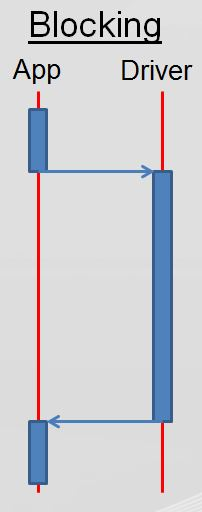
\includegraphics[width=.4\linewidth]{BlockingSequence}
  \caption{Comportamento blocante}
  \label{fig:sub1}
\end{subfigure}%
\begin{subfigure}[b]{.5\textwidth}
  \centering
  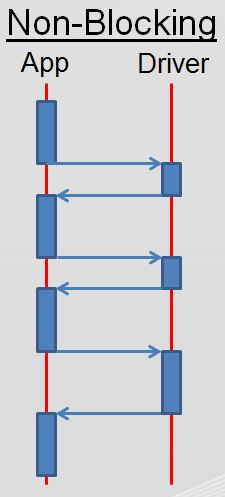
\includegraphics[width=.4\linewidth]{NonBlockingSequence}
  \caption{Comportamento não-blocante}
  \label{fig:sub2}
\end{subfigure}
\caption{Comparação entre comportamento blocante e não-blocante}
\label{fig:test}
\end{figure}

\par Kits de desenvolvimento para microcontroladores que ajudam a abstrair a implementação do
hardware do programador são sempre benéficos por tornarem o processo de desenvolvimento de
aplicações para aquele módulo mais simples e acessível. Microcontroladores Arduino são
normalmente programados em um ambiente de linguagem C, uma linguagem procedural, e os drivers
e bibliotecas disponibilizados pela própria Arduino apresentam atualmente funções e módulos que
causam o bloqueio da aplicação por utilizarem a técnica de polling. Embora existam reimplementações
por parte da comunidade de alguns desses módulos de forma a eliminar o bloqueio, Céu-Arduino
ainda não possui bibliotecas implementadas em Céu que resolvam o problema.
\par O kit de desenvolvimento Céu-Arduino apresenta uma abordagem única para o desenvolvimento
orientado a eventos e suporte a interrupções, e se encontra atualmente em um estado inicial. O
projeto está em uma versão 0.20 e conta com exemplos básicos de aplicações em Arduino queutilizam a linguagem Céu. Apesar de não possuir somente poucas bibliotecas e drivers desenvolvidos
em Céu, a linguagem é de fácil integração com C, sendo possível utilizar os módulos desenvolvidos
atualmente para Arduino. \cite{githubceuarduino}

\section{Proposta e Objetivos do Trabalho}
\tab O projeto tem como objetivo implementar no ambiente Céu-Arduino bibliotecas e drivers que
sirvam como alternativa aos bloqueantes utilizados atualmente. Módulos atuais serão estudados de
forma a definir-se quais serão reimplementados, com foco na pertinência de tais funcionalidades para
aplicações em sistemas embarcados, mais especificamente nas áreas de sistemas distribuído e redes
de sensores e atuadores. Bibliotecas de Arduino de protocolos de comunicação, como Wire, e de
leitura de valores analógicos, como Analog I/O, seriam exemplos de módulos cuja reimplementação
atenderia o requisito de pertinência mencionado.
\par A abordagem escolhida para implementação será modelar as funções de forma que a aplicação não
bloqueie e sim aguarde a emissão de um evento que marca a mudança de estado do hardware pelas
flags, disparando a interrupção e executando a rotina associada ao estado do hardware dentro da
execução da funcionalidade.
\par Os módulos serão desenvolvidos com o objetivo de serem uma contribuição para o projeto Céu-
Arduino e a comunidade de sistemas embarcados. Por esse motivo, sua implementação será dada
com o acompanhamento do gestor do projeto Céu-Arduino, de modo a respeitar os padrões
desejados e previstos.
\par Espera-se que durante o processo de desenvolvimento seja estabelecido um framework reproduzível
para implementação de bibliotecas e drivers em Céu-Arduino, e que tal possa ser utilizado para
facilitar o trabalho de futuros desenvolvedores. O processo será documentado com esse objetivo em
mente.
\par Uma aplicação em Sistemas Distribuídos será feita, por fim, de modo a servir como objeto de teste e
estudo das bibliotecas e drivers implementados. Espera-se que os dados coletados mostrem
claramente as vantagens da utilização de versões não-bloqueantes dos módulos. Embora ainda não
tenha seu escopo definido por completo, a aplicação envolverá uma rede de sensores e atuadores, de
modo a demonstrar os módulos implementados de interface com sensores e atuadores, como o Wire
para dispositivos I2C e Analog I/O para sensores e atuadores analógicos. Os componentes irão
utilizar protocolos de troca de mensagens para transmitirem informação e se sincronizarem. O uso
das novas chamadas não-bloqueantes permitirá à aplicação melhor realizar seus ciclos
computacionais para realizar essas tarefas, já que os ciclos antes gastos com polling dos drivers de
sensores e atuadores será utilizado para processamento dos dados e mensagens.
\par Como os exemplos dados na introdução (sistema de iluminação inteligente; sistema de irrigação
monitorada; um controlador de tráfego), busca-se uma estrutura onde existem unidades distribuídas
pelo ambiente responsáveis por coleta de informação e / ou realização de ações, trocando
informação e se sincronizando por troca de mensagens. Essa é uma boa estrutura para exemplificar
os módulos desenvolvidos pois os sensores e atuadores justificarão o uso das novas interfaces não
bloqueantes, liberando a aplicação para processar os dados coletados e trocar mensagens com
eficiência de modo a manter a sincronização e estabilidade do sistema a um menor consumo de
energia.
\section{Atividades Realizadas}
\tab Como primeira etapa do projeto foram definidos os módulos para os quais implementações não-
bloqueantes em Céu serão desenvolvidas. Os módulos são Entrada e Saída Analógica (Analog
I/O), Comunicação SPI (SPI), Comunicação Serial (Serial), Suporte a RTC Externo
(External RTC) e Operações na EEPROM (EEPROM). Os módulos foram descritos na ordem
estimada de dificuldade crescente.
\par O realizado dentro desta primeira etapa do projeto girou em torno do desenvolvimento de um dos
módulos. Para que o driver fosse implementado, foi necessário um estudo não só da plataforma
Arduino e do microcontrolador, mas também do ambiente de desenvolvimento disponibilizado pela
AVR e das bibliotecas já implementadas e disponibilizadas em Céu, principalmente as de Céu-
Arduino.
\par Todo o código desenvolvido neste projeto segue a intenção de priorizar simplicidade e rapidez na
execução, respeitando os requisitos de um módulo suficientemente robusto e funcional. De tal
modo, os drivers desenvolvidos atenderão somente a plataforma Arduino Uno, por ser a mais
utilizada e disponível, além de possuírem limitações que podem vir a exigir atenção e
responsabilidade do usuário final no uso dos drivers em aplicações. O motivo é a busca por uma
melhor utilização do tempo do projeto e redução da carga computacional para a execução dos drivers.
\par Ao final desta etapa, o projeto se encontra com um driver já desenvolvido e em uma versão estável.
Tal módulo servirá como base para que o processo de desenvolvimento possa ser reproduzido para
os demais drivers. A explicação de cada etapa nesta sessão do relatório virá acompanhada do exemplo
prático da implementação referente ao módulo. Deste modo, o processo será descrito assim como o
desenvolvimento do driver.
\par O módulo desenvolvido nesta primeira etapa do projeto é o de leitura e emissão de valores de
voltagem analógicos. A referência para este módulo no texto daqui em diante será “Analog I/O”,
significando “Entrada e Saída Analógica”.

\subsection{Estudo do Ambiente de Desenvolvimento C}

\tab O ambiente de desenvolvimento que usa a linguagem C é o mesmo tanto para Arduino quanto para
Céu-Arduino. Isto é, ambos os códigos são em alguma etapa compilados utilizando o mesmo
compilador. Esse compilador é disponibilizado pela AVR e é uma versão customizada de GCC,
chamada de AVR-GCC. Em conjunto com o compilador, são utilizadas bibliotecas da AVR que
tratam da abstração do hardware, como acesso a registradores, para variados chips da Atmel, incluindo
o AtMega328p, presente no Arduino Uno, plataforma para qual os módulos deste projeto são
destinados.
\par Outra ferramenta essencial para o andamento do projeto é a capacidade de se registrar rotinas de
serviço a interrupções (Interrupt Service Routines, ISR), que são rotinas de código associadas a
interrupções do microcontrolador. Em outras palavras, quando o hardware emite uma interrupção, osoftware executaria a ISR atrelada àquela interrupção. AVR disponibiliza uma biblioteca de tratamento
de interrupções que torna simples a implementação de tais ISRs.
\par Para Analog I/O, isso significa que teremos fácil acesso a quaisquer registradores atrelados ao
módulo, e o acesso ao hardware ficará transparente para o desenvolvedor, que irá tratar os
registradores como vetores de bits. Como será mencionado posteriormente, isso procede tanto para
o ambiente de desenvolvimento C quanto o ambiente Céu.

\subsection{Estudo do Hardware}

\tab AVR disponibiliza um documento detalhado \cite{wortmann2015} das especificações do microcontrolador presente no
Arduino Uno, o AtMega328p. Esse documento, chamado datasheet, possui a definição de todas as
funcionalidades e hardwares dedicados presentes, incluindo a definição e descrição dos registradores
responsáveis e atrelados a cada um. Esse documento é vital para o entendimento das capacidades e
limitações do chip e, principalmente, o de como operá-lo.
\par A datasheet está no centro da primeira etapa do desenvolvimento, que é estudar o funcionamento do
hardware para que, em conjunto com o estudo do código da implementação atual (se existente), seja
possível compreender o comportamento de uma API tradicional. O foco desse passo é criar uma
base de conhecimento sobre as informações já disponíveis acerca do módulo.
\par Durante essa etapa no desenvolvimento do Analog I/O, foi levantado que as funcionalidades de
entrada (leitura de valor analógico) e saída (emissão de valor analógico) são atreladas a hardwares
dedicados distintos no microcontrolador. Enquanto os valores de saída analógicos são simulados
utilizando ondas PWM (o pino liga e desliga em intervalos regulares, onde o valor analógico seria a
razão entre o tempo que permanece ligado e o tempo que permanece desligado). Essa funcionalidade
já se encontra implementada em Céu e, portanto, não é pertinente para os efeitos deste relatório.
\par Os valores de leitura, em outra mão, são obtidos por um hardware de Conversão Analógica para
Digital (ADC). Esse componente dedicado recebe um valor de voltagem analógico e, após ciclos de
processamento, guarda em seus registradores a representação de 10 bits deste valor, quando
comparado a uma referência de valor máximo. Em outras palavras, se a voltagem de entrada for o
ground, o resultado será “0”. Caso seja igual ou acima da voltagem de referência, será 1023.
\par Embora existam mais de um pino de leitura analógico no microcontrolador, existe somente um
hardware de ADC. Para que possa atender a todos os seis pinos, o hardware conta com um
multiplexador que seleciona o pino para qual a leitura deve ser feita. Repare que não é possível ter
mais de um pino tendo seu valor lido pelo hardware ao mesmo tempo. O valor desse multiplexador se
encontra em um dos registradores ao qual o desenvolvedor possui acesso e, portanto, seu valor pode
ser modificado facilmente. Além do multiplexador, o usuário possui acesso a vários valores que
servem como configuração do ADC. Dentre esses valores, o de Analog to Digital Interrupt
Enable (ADIE) é de elevado interesse ao projeto, já que quando este bit, presente no registrador de
configuração ADCSRA, se encontra “setado” (valor lógico 1), o hardware dispara uma interrupção
toda vez que uma conversão termina.
\par Em resumo, para efetuar uma conversão, o multiplexador, cujo valor é controlado pelo registrador
ADMUX, deve receber o valor do pino para qual a leitura será feita. Do mesmo modo, os outros
bits de configuração devem ser setados de acordo com a configuração desejada pelo usuário. Para
iniciar a conversão, basta que o software escreva o valor lógico 1 no bit ADSC. Esse bit terá seu valor
1 mantido pelo hardware enquanto a conversão está em progresso, e será zerado no momento que a
conversão tiver fim e o resultado estiver disponível. Os nomes técnicos dos bits e registradores serão
referenciados no texto quando descrevendo a implementação.

\subsection{Implementação Original}

\tab A implementação atual de uma função de leitura analógica, presente na biblioteca de funções
disponibilizada pela Arduino, possui como único argumento o pino para qual a conversão deve ser
feita, devolvendo o resultado da mesma.
\par A função configura os registradores do hardware, incluindo ADMUX, cujo valor terá como base o
argumento de entrada da função. Em seguida, inicia a conversão escrevendo o lógico 1 em ADSC.
Para aguardar o fim da conversão, o código faz polling em ADSC. Como já discutido, isso caracteriza
o motivo da aplicação apresentar um comportamento bloqueante, e é o que o projeto visa eliminar.
Após ADSC ter sido zerado pelo hardware, a função segue sua execução e retorna o valor do
resultado.
\subsection{Implementação Mínima Viável}
\tab Após a funcionalidade ter sido estudada do ponto de vista do hardware e do software (caso este seja
disponível), a causa do comportamento bloqueante da aplicação deverá ter sido identificada e uma
solução idealizada. Essa solução pode ter como base a capacidade do hardware de gerar interrupções
ou quaisquer outros métodos para que não seja necessário à aplicação consultar o hardware, e sim
cadastrar um call-back para que o modelo de Céu funcione.
\par Com base na solução, deverá ser implementada uma API na linguagem de escolha. No âmbito deste
projeto, essa linguagem será C. Embora possa não se assemelhar com a implementação final, essa
solução intermediária deve apresentar contribuições claras ao código final, mesmo que na forma de
aprendizado.
\par A implementação em C do driver para gerenciar o ADC buscou eliminar o polling encontrado (descrito
na última sessão) utilizando a capacidade do módulo de emitir uma interrupção quando a conversão
for concluída e o registro de uma ISR atrelada a essa interrupção utilizando as utilidades
disponibilizadas pela AVR.
\par A implementação nova reaproveita a implementação original, modificando a lógica do polling.
Enquanto a original possuía apenas uma função que encapsulava todo o processo de leitura, desde a
configuração do hardware dedicado até o retorno do valor, a API nova é dividida em três funções, que
contam com o suporte de uma ISR atrelada à interrupção do ADC e uma variável global que guarda
o estado de uma conversão.
\par A primeira função é equivalente à função de leitura da implementação original até o momento do
início da conversão, isto é, ela termina quando ADSC recebe o valor lógico 1. Entretanto ela
configura ADIE para que as interrupções ocorram, algo que não estava previsto na implementação
da Arduino. Essa função altera o valor da variável de estado para que esta reflita que uma conversão
está em andamento.
\par A segunda função é utilizada para consultar a variável de estado de modo a saber se uma conversão
está acontecendo. Isso é necessário pois caso esteja, os valores contidos nos registradores que
guardam o resultado da conversão podem não ser verdadeiros.
\par A terceira função é equivalente à parte final da função da implementação original, após o polling. Ela
simplesmente retorna o resultado da conversão contido nos registradores.
\par A ISR atrelada à interrupção do ADC altera o valor da variável de estado para refletir que uma
interrupção terminou.
\par Para efetuar uma leitura de um valor analógico utilizando esta API, o usuário deve chamar a primeira
função para iniciar a conversão e, depois que a segunda função retorne um valor negativo
(representando que uma conversão não está em progresso), chamar a terceira função para obter o
resultado.

\subsection{Estudo do Ambiente de Desenvolvimento Céu}

\tab A linguagem Céu permite uma forte integração com C, sendo capaz de chamar funções e acessar
variáveis declaradas e contidas no contexto C. Isso permite que parte da implementação mínima
viável seja reutilizado no desenvolvimento da versão da API em Céu. O ambiente também permite a
declaração de ISRs, o que torna possível reproduzir a API em C dentro do ambiente Céu desde o
primeiro momento.
\par A vantagem de Céu é a modelagem orientada a eventos, o que permite que a API execute baseada
em call-backs, contribuindo para a eliminação do desperdício dos ciclos (que eram utilizados para
checar se a API e encontrava em um estado que permitia a próxima ação). Este passo no
desenvolvimento deve ser utilizado para modelar a solução concebida nos passos anteriores de forma
que utilize as vantagens de Céu a favor da economia de ciclos, implementando a estrutura de
orientação a eventos prevista no modelo Céu.
\par Nesta etapa do desenvolvimento do módulo ADC, a obtenção do resultado da conversão foi
modelada como um evento emitido pelo driver. Deste modo, a API consiste na requisição de uma
conversão por parte da aplicação e da emissão, por parte da API, de um evento que carrega o
resultado.

\subsection{Implementação em Céu}

\tab Após ter a API modelada em Céu, o desenvolvedor possuiu todas as ferramentas para produzir a
solução final. Deve-se buscar tirar o máximo de proveito possível do trabalho realizado nas etapas
anteriores.
\par A implementação em Céu do módulo ADC constituiu ter uma função que iniciava uma conversão,
função esta que foi reaproveitada da API em C. Como a própria API será responsável por emitir o
resultado quando a conversão terminar, não há necessidade de manter uma variável de estado. Basta
que, na ISR, o resultado seja obtido utilizando a função implementada no passo anterior e que este
valor seja enviado à aplicação na forma de um evento. Todo o controle de estados do driver é
encapsulado pelo próprio modelo de Céu e o fluxo de execução.
\par Para efetuar uma conversão, a aplicação, agora em Céu, deve requisitar uma conversão e “aguardar”
o evento resultado. Como previsto no ambiente Céu, enquanto a aplicação está “aguardando” o
evento, o microcontrolador fica livre para executar outras linhas de código pendentes ou, caso
nenhuma exista, entrar em um estado de baixo consumo de energia. Quando o hardware concluir a
conversão, o evento emitido irá “acordar” a aplicação, que seguirá seu fluxo. No caso da
implementação original, a aplicação não poderia fazer uso desse tempo de “aguarde” pois estaria
bloqueada consultando o driver para saber se a conversão já havia terminado. O contraste entre as
duas aplicações e, por consequência, o contraste entre as duas APIs ficam claros.

\section{Revisão do Plano de Ação}

\tab Embora o planejamento original previsse um estudo de todos os módulos antes da implementação,
foi percebido que tratar cada módulo separadamente é mais vantajoso em termos de aprendizado e
produtividade, visto que o estudo e modelagem da solução para cada módulo é independente dos
outros módulos. Além disso, implementar uma API por completo promove experiência que será útil
no desenvolvimento das soluções seguintes.
\par Deste modo, embora as etapas previstas anteriormente para todos os módulos permanecem
pertinentes, elas serão realizadas dentro do âmbito de cada módulo. O novo planejamento e
cronograma, para evitar redundâncias, será dividido por módulo.
\par Segue o novo planejamento e explicação breve das etapas e objetivos esperados para o cumprimento
do projeto:
\begin{itemize}

\item Definição dos módulos. Serão definidos quais módulos serão implementados em Céu ao
longo do projeto.
\item Desenvolver módulo. Para cada um dos cinco módulos propostos:
\begin{itemize}

\item Aprofundamento no estado da arte. Será estudada a implementação atual de
biblioteca e driver de Arduino que causam o bloqueio da aplicação. Serão estudadas
as implementações de bibliotecas e drivers em Céu, de modo a melhor conhecer o
padrão proposto pela linguagem.
\item Estudo do hardware. Análise baixo-nível das consequências do código em C da
plataforma Arduino de modo a entender como o microcontrolador reage, utilizando
datasheet como referência.
\item Elaborar alternativas e soluções. Planos de ação para uma implementação não-
bloqueante.
\item Implementação dos módulos. Serão desenvolvidos o driver e biblioteca, em conjunto
com aplicação que exemplifique suas funcionalidades.
\item Documentação dos módulos. O módulo desenvolvido sofrerá quaisquer ajustes
necessários para que siga o padrão previsto em Céu-Arduino e esteja considerado
pronto para uso. Toda modificação ao módulo a partir deste ponto deve ser mínima
visto que a etapa de desenvolvimento do mesmo deve ser dada como completa.

\end{itemize}

\item Definição do escopo da aplicação. A aplicação deve ser capaz de demonstrar as vantagens da
reimplementação de cada módulo desenvolvido. A aplicação envolverá comunicação entre
módulos independentes a fim de sincronização como esperado de uma aplicação de sistemas
distribuídos.
\item Desenvolvimento da aplicação. Deve ser desenvolvida e modelada de modo que seja viável a
coleta de dados.
\item Análise dos dados e relatório. Com base na análise dos dados será feito um relatório
demonstrando as vantagens e proponho melhorias para os módulos desenvolvidos.

\end{itemize}

\section{Cronograma}

\begin{center}
\begin{tabular}{|c|c|c|c|c|c|c|c|c|}
\hline
&Mês 1&Mês 2&Mês 3&Mês 4&Mês 5&Mês 6&Mês 7&Mês 8 \\
\hline
Definição dos módulos & \cellcolor[HTML]{808080} &&&&&&& \\
\hline
Desenvolver módulo Analog I/O & \cellcolor[HTML]{808080} & \cellcolor[HTML]{808080} &&&&&& \\
\hline
Desenvolver módulo SPI && \cellcolor[HTML]{808080} & \cellcolor[HTML]{808080} &&&&& \\
\hline
Desenvolver módulo Serial &&& \cellcolor[HTML]{808080} & \cellcolor[HTML]{808080} &&&& \\
\hline
Desenvolver módulo External RTC &&&& \cellcolor[HTML]{808080} & \cellcolor[HTML]{808080} &&& \\
\hline
Desenvolver módulo EEPROM &&&&& \cellcolor[HTML]{808080} & \cellcolor[HTML]{808080} && \\
\hline
Definir escopo da aplicação &&&&&& \cellcolor[HTML]{808080} && \\
\hline
Desenvolver a aplicação &&&&&&& \cellcolor[HTML]{808080} & \cellcolor[HTML]{808080}  \\
\hline
Análisar dados e produzir relatório &&&&&&&& \cellcolor[HTML]{808080}  \\
\hline
\end{tabular}
\end{center}

\newpage

\printbibliography

\end{document}
